% ---------------------------------------------------------------
% TEMPLATE TCC1 - SENAC SANTO AMARO
% ---------------------------------------------------------------
% Trabalho de Conclusão de Curso 1
% Elaborado para apresentação da proposta inicial do TCC
% Estrutura: 4 capítulos (Introdução, Revisão Bibliográfica,
%            Desenvolvimento, Referências Bibliográficas)
% ---------------------------------------------------------------

\documentclass[
    12pt,                % tamanho da fonte
    openright,           % capítulos começam em página ímpar
    oneside,             % para impressão em apenas um lado do papel
    a4paper,             % tamanho do papel
    english,             % idioma adicional
    brazil               % idioma principal
]{abntex2}

% ---------------------------------------------------------------
% PACOTES
% ---------------------------------------------------------------
\usepackage{lmodern}                % Fonte Latin Modern
\usepackage[T1]{fontenc}            % Seleção de códigos de fonte
\usepackage[utf8]{inputenc}         % Codificação do documento
\usepackage{lastpage}               % Usado pela Ficha catalográfica
\usepackage{indentfirst}            % Indenta o primeiro parágrafo
\usepackage{color}                  % Controle de cores
\usepackage{graphicx}               % Inclusão de gráficos
\usepackage{microtype}              % Melhorias de justificação
\usepackage{float}                  % Para posicionamento de figuras
\usepackage{booktabs}               % Tabelas profissionais
\usepackage{multirow}               % Células mescladas em tabelas
\usepackage{longtable}              % Tabelas longas
\usepackage{amsmath,amssymb}        % Símbolos matemáticos
\usepackage{pgfgantt}               % Diagramas de Gantt
\usepackage[brazilian,hyperpageref]{backref}  % Páginas com citações
\usepackage[alf]{abntex2cite}       % Citações ABNT

% ---------------------------------------------------------------
% CONFIGURAÇÕES DO PDF
% ---------------------------------------------------------------
\makeatletter
\hypersetup{
    pdftitle={\@title},
    pdfauthor={\@author},
    pdfsubject={TCC1 - SENAC Santo Amaro},
    pdfcreator={LaTeX with abnTeX2},
    pdfkeywords={tcc}{senac}{santo amaro}{trabalho de conclusão},
    colorlinks=true,        % false: links em caixas; true: links coloridos
    linkcolor=blue,         % cor dos links internos
    citecolor=blue,         % cor dos links para bibliografia
    filecolor=magenta,      % cor dos links para arquivos
    urlcolor=blue,
    bookmarksdepth=4
}
\makeatother

% ---------------------------------------------------------------
% CONFIGURAÇÕES DE APARÊNCIA DO PDF FINAL
% ---------------------------------------------------------------
\definecolor{blue}{RGB}{41,5,195}

% ---------------------------------------------------------------
% INFORMAÇÕES DO DOCUMENTO
% ---------------------------------------------------------------
\titulo{Sistema Inteligente de Tradução de Libras Utilizando Visão Computacional e Processamento de Linguagem Natural}
\autor{Júlia Almeida Leite \\ Maria Eduarda Mariano Coelho}
\local{São Paulo}
\data{2026}
\orientador{Prof. Thyago Conchado Quintas}
% \coorientador{Prof. Nome do Coorientador} % Descomente se houver coorientador

\instituicao{%
  SENAC -- Serviço Nacional de Aprendizagem Comercial
  \par
  Unidade Santo Amaro
  \par
  Curso de Bacharelado em Ciência da Computação
}

\tipotrabalho{Trabalho de Conclusão de Curso I}

\preambulo{Proposta de Trabalho de Conclusão de Curso apresentado ao SENAC Santo Amaro como requisito parcial para aprovação na disciplina de TCC1 do curso de Bacharelado em Ciência da Computação.}

% ---------------------------------------------------------------
% COMPILA O ÍNDICE
% ---------------------------------------------------------------
\makeindex

% ---------------------------------------------------------------
% INÍCIO DO DOCUMENTO
% ---------------------------------------------------------------
\begin{document}

% Seleciona o idioma do documento
\selectlanguage{brazil}

% Retira espaço extra obsoleto entre as frases
\frenchspacing

% ---------------------------------------------------------------
% ELEMENTOS PRÉ-TEXTUAIS
% ---------------------------------------------------------------
\pretextual

% ---------------------------------------------------------------
% CAPA
% ---------------------------------------------------------------
\imprimircapa

% ---------------------------------------------------------------
% FOLHA DE ROSTO
% ---------------------------------------------------------------
\imprimirfolhaderosto

% ---------------------------------------------------------------
% RESUMO
% ---------------------------------------------------------------
\begin{resumo}
Este documento apresenta a proposta inicial do Trabalho de Conclusão de Curso (TCC1) desenvolvido no SENAC Santo Amaro. O objetivo deste trabalho é [descrever brevemente o objetivo principal do TCC]. A justificativa para este estudo baseia-se em [descrever brevemente a justificativa]. A revisão bibliográfica abrange [mencionar os principais tópicos]. Como solução proposta, pretende-se [descrever brevemente a solução]. Este trabalho está organizado em três capítulos que apresentam a introdução ao tema, a revisão bibliográfica que fundamenta a pesquisa, o desenvolvimento com a solução proposta e o cronograma de trabalho, seguidos das referências bibliográficas.

\vspace{\onelineskip}

\noindent
\textbf{Palavras-chave}: palavra1. palavra2. palavra3. palavra4. palavra5.
\end{resumo}

% ---------------------------------------------------------------
% LISTA DE ILUSTRAÇÕES
% ---------------------------------------------------------------
% \pdfbookmark[0]{\listfigurename}{lof}
% \listoffigures*
% \cleardoublepage

% ---------------------------------------------------------------
% LISTA DE TABELAS
% ---------------------------------------------------------------
% \pdfbookmark[0]{\listtablename}{lot}
% \listoftables*
% \cleardoublepage

% ---------------------------------------------------------------
% SUMÁRIO
% ---------------------------------------------------------------
\pdfbookmark[0]{\contentsname}{toc}
\tableofcontents*
\cleardoublepage

% ---------------------------------------------------------------
% ELEMENTOS TEXTUAIS
% ---------------------------------------------------------------
\textual

% ===============================================================
% CAPÍTULO 1 - INTRODUÇÃO
% ===============================================================
\chapter{Introdução}
\label{cap:introducao}
A comunicação é extremamente importante para promover a inclusão social. No entanto, muitas pessoas surdas que utilizam a Língua Brasileira de Sinais (Libras) encontram barreiras na interação com aqueles que não conhecem essa linguagem. Essa limitação afeta diretamente o acesso a serviços, educação e oportunidades do dia a dia.

O desafio da comunicação reside no fato de que a Libras e a Língua Portuguesa possuem modalidades distintas sendo esta oral-auditiva e linear, e aquela visual-espacial e simultânea \cite{Olizaroski2024}. Enquanto o português organiza os elementos da frase em sequência fixa, a Libras expressa informações por meio da combinação simultânea de configurações de mão, movimentos e expressões faciais, com ordem frasal flexível que varia conforme o contexto comunicativo \cite{Quadros2004}.

Com a evolução das tecnologias em inteligência artificial, surgem novas maneiras de diminuir essas barreiras. O desenvolvimento do trabalho proposto apoia-se em quatro eixos tecnológicos complementares.

O primeiro eixo é a visão computacional, responsável por capturar e interpretar os sinais a partir do fluxo de vídeo da câmera. Nesse processo, a ferramenta MediaPipe \cite{Lugaresi2019} desempenha o papel central ao detectar, com o processamento ao vivo, os 21 pontos-chave (\textit{landmarks}) das articulações da mão, fornecendo coordenadas tridimensionais que descrevem a geometria e o movimento dos sinais de forma compacta e independente de variações de iluminação ou tom de pele \cite{Zhang2020}.

O segundo eixo é o aprendizado profundo (\textit{deep learning}), que fornece a base para o reconhecimento dos sinais a partir dessas representações visuais. Para sinais estáticos, como as configurações do alfabeto manual, são empregadas Redes Neurais Convolucionais (CNN), capazes de identificar padrões espaciais nas configurações de mão \cite{Lecun1998}. Para sinais dinâmicos, cuja compreensão depende da trajetória e da sequência de movimentos ao longo do tempo, utilizam-se Redes de Memória de Longo Prazo (LSTM), arquitetura especializada no processamento de sequências temporais \cite{Hochreiter1997}.

O terceiro eixo é o processamento de linguagem natural (NLP), que atua como uma camada de conversão inteligente entre as saídas do reconhecedor de gestos e o texto intermediário em português. Sua função é interpretar os sinais isolados identificados pela visão computacional e reorganizá-los semântica e sintaticamente, realizando os ajustes de concordância e ordem frasal necessários para transformar a estrutura própria da Libras em frases coerentes e gramaticalmente corretas. Para isso, o módulo de NLP, implementado com a biblioteca spaCy, utiliza árvores de dependência sintática para identificar as relações gramaticais entre os \textit{tokens} (sujeito, verbo e objeto) e reconstituir a sentença na estrutura do português \cite{Jurafsky2023}.

O quarto eixo é o uso de um Modelo de Linguagem de Grande Escala (LLM, do inglês \textit{Large Language Model}), responsável por refinar e contextualizar a saída produzida pelo módulo de NLP. Após a reorganização sintática inicial, o LLM recebe a frase intermediária e aplica conhecimento linguístico profundo para corrigir ambiguidades, inserir artigos e preposições ausentes e produzir uma sentença final fluente em português \cite{Brown2020}.

O sistema será treinado e validado sobre três bases de dados de Libras: o MINDS-Libras \cite{Rezende2021}, o V-Librasil \cite{Rodrigues2021} e o Libras Brazilian Sign Language \cite{Pas2020}, selecionados pela diversidade de sinalizadores, vocabulário e modalidade de captura. O desempenho da solução será avaliado por métricas complementares: a acurácia e a matriz de confusão para o módulo de reconhecimento gestual, a métrica BLEU para a qualidade linguística das traduções geradas, e a latência para verificar a adequação do sistema ao uso em tempo de execução.

É importante ressaltar que, devido à amplitude lexical da Libras e à natureza experimental deste estudo, o sistema proposto não visa uma tradução universal imediata. A pesquisa delimita-se ao reconhecimento de um conjunto inicial de sinais voltados a contextos específicos, para garantir o rigor técnico na integração entre os quatro eixos, estabelecendo um modelo de referência que possa, em etapas posteriores, ser expandido para um léxico mais abrangente.

Diante disso, este trabalho propõe desenvolver um sistema de tradução de Libras que articula visão computacional, aprendizado profundo, processamento de linguagem natural e modelos de linguagem de grande escala em um \textit{pipeline} integrado. O objetivo é contribuir para a inclusão social com uma solução acessível e aplicável em contextos como atendimentos, ambientes educacionais e interações cotidianas.

% ---------------------------------------------------------------
\section{Contexto}
\label{sec:contexto}

A comunicação é necessária para a integração social e o exercício da cidadania. Contudo, para a comunidade surda no Brasil, essa interação muitas vezes é limitada por barreiras linguísticas significativas. Conforme dados do \cite{IBGE2019}, o Brasil conta com mais de 10 milhões de pessoas com algum nível de deficiência auditiva, sendo cerca de 2,3 milhões completamente surdas. 

% ---------------------------------------------------------------
\section{Justificativa}
\label{sec:justificativa}

A comunicação é fundamental para a inclusão social e para a participação das pessoas na sociedade. No Brasil, embora a Língua Brasileira de Sinais (Libras) seja reconhecida oficialmente, ainda existem dificuldades na comunicação entre pessoas surdas e ouvintes. Um dos principais motivos é o número reduzido de pessoas que conhecem a língua, o que acaba limitando interações no dia a dia. Diante disso, torna-se importante pensar em alternativas que utilizem tecnologia para facilitar essa comunicação e tornar o acesso mais inclusivo.

Do ponto de vista acadêmico, este trabalho se insere na área de Ciência da Computação ao combinar técnicas de visão computacional e processamento de linguagem natural em uma mesma solução. Trata-se de um problema que não é simples, pois envolve desde o reconhecimento de movimentos e gestos até a construção de frases compreensíveis em português. Além disso, lidar com dados visuais em sequência e interpretar corretamente os sinais são desafios relevantes, o que torna a proposta interessante como estudo e desenvolvimento na área de inteligência artificial aplicada.

Em relação à prática, a proposta pode trazer benefícios concretos, principalmente para a comunidade surda. Um sistema capaz de traduzir Libras automaticamente pode ajudar a diminuir a dependência de intérpretes em situações cotidianas, como atendimentos, ambientes educacionais ou interações básicas. Com isso, há um ganho em autonomia e acessibilidade, além de ampliar as possibilidades de comunicação em diferentes contextos.

Apesar de já existirem pesquisas nessa área, ainda há aspectos que podem ser melhor explorados. Muitos trabalhos focam no reconhecimento de sinais isolados, sem considerar de forma mais ampla o contexto da comunicação. Outros utilizam bancos de dados específicos, relacionados à representação das variações da Libras. Além disso, ainda são limitados os estudos que integram todo o processo, desde a identificação dos gestos até a formação de frases com sentido em português.

Portanto, este trabalho busca avançar nesse quesito ao propor uma solução mais integrada, que não se limite apenas ao reconhecimento individual de sinais, mas que também considere a construção da linguagem. A intenção é contribuir tanto para a área acadêmica quanto para a sociedade, explorando uma aplicação prática da inteligência artificial voltada à acessibilidade.

% ---------------------------------------------------------------
\section{Objetivo}
\label{sec:objetivo}

Os objetivos deste trabalho estão voltados para o desenvolvimento de uma solução capaz de auxiliar na comunicação entre pessoas surdas e ouvintes por meio da tradução automática de Libras. Para isso, define-se um objetivo principal que orienta a proposta geral do sistema, enquanto os objetivos secundários detalham as etapas necessárias para sua construção, incluindo desde o tratamento dos dados até a implementação e avaliação da solução.

\subsection{Objetivo principal}

Implementar um sistema computacional capaz de reconhecer gestos da Língua Brasileira de Sinais (Libras) por meio de visão computacional e traduzi-los em frases gramaticalmente coerentes em língua portuguesa, utilizando técnicas de processamento de linguagem natural e modelos de linguagem de grande escala.

\subsection{Objetivos secundários}

\begin{enumerate}
    \item Realizar levantamento bibliográfico sobre reconhecimento de gestos em Libras, arquiteturas de redes neurais convolucionais e recorrentes, processamento de linguagem natural e modelos de linguagem de grande escala aplicados à tradução automática;
    \item Selecionar, estruturar e pré-processar os datasets de Libras, aplicando técnicas de balanceamento e augmentação de dados para garantir a qualidade do treinamento;
    \item Projetar a arquitetura híbrida do sistema, integrando o módulo de visão computacional baseado em MediaPipe, CNN e LSTM ao módulo de NLP implementado com spaCy e refinamento via LLM;
    \item Implementar um protótipo funcional do pipeline completo de tradução, desde a captura de vídeo via webcam até a exibição da frase traduzida em português na interface do usuário;
    \item Validar o desempenho do sistema por meio de métricas quantitativas de acurácia e matriz de confusão para o módulo de reconhecimento gestual, métrica BLEU para a qualidade linguística das traduções, e análise de latência para verificar a viabilidade do uso em tempo real.
\end{enumerate}

% ===============================================================
% CAPÍTULO 2 - REVISÃO BIBLIOGRÁFICA
% ===============================================================
\chapter{Revisão Bibliográfica}
\label{cap:revisao}

Neste capítulo, são apresentados os conceitos fundamentais necessários para o entendimento do projeto. Inicialmente, são abordadas as diferenças estruturais entre a Língua Brasileira de Sinais (Libras) e a Língua Portuguesa. Em seguida, são apresentados os fundamentos de visão computacional aplicados ao reconhecimento de gestos e o uso de redes neurais. Por fim, são discutidos conceitos de processamento de linguagem natural, que servirão como base para a construção de frases em português a partir dos sinais identificados.

% ---------------------------------------------------------------
\section{Referencial teórico}
\label{sec:referencial}

Esta seção apresenta os conceitos fundamentais que embasam o desenvolvimento do sistema proposto, organizados de acordo com os eixos tecnológicos do projeto: a língua alvo da tradução, os dados necessários para o treinamento, a cadeia de visão computacional e as abordagens de linguagem natural. Cada tópico é tratado em seu aspecto conceitual e científico, fornecendo a base teórica para as decisões de arquitetura e implementação detalhadas na seção de Fundamentos.
 
\subsection{Linguagem da Língua Brasileira de Sinais (Libras)}
 
A Língua Brasileira de Sinais (Libras) é uma língua natural, completa e autônoma, utilizada pela comunidade surda no Brasil, reconhecida pela Lei nº 10.436/2002 e regulamentada pelo Decreto nº 5.626/2005 como meio legal de comunicação e expressão. Possui estrutura gramatical própria, independente da Língua Portuguesa, e está inserida em um contexto cultural e linguístico específico da comunidade surda.
 
Do ponto de vista linguístico, a Libras pertence à modalidade visual-espacial, em contraste com a modalidade oral-auditiva do português. Essa diferença implica mudanças importantes na forma como a informação é organizada: enquanto a língua portuguesa apresenta uma estrutura linear, em que os elementos aparecem em sequência, a Libras permite expressar diferentes informações ao mesmo tempo, por meio da combinação de sinais, movimentos e expressões faciais.
 
As expressões faciais e corporais possuem papel fundamental na Libras, não sendo utilizadas apenas para transmitir emoções, mas também como elementos gramaticais da língua. Conhecidas como Expressões Não Manuais (ENM), elas complementam os sinais realizados com as mãos e auxiliam na construção do significado das frases \cite{Quadros2004}. Em muitos casos, a ausência dessas expressões pode dificultar a compreensão ou até alterar o sentido do enunciado.
 
Diferentes movimentos do rosto podem indicar intenções comunicativas específicas. Expressões faciais associadas ao movimento das sobrancelhas, por exemplo, podem marcar perguntas, negações e intensificações, funcionando como elementos linguísticos da estrutura da Libras \cite{Brito1995}. Além disso, movimentos da boca, direção do olhar e expressões corporais também contribuem para a construção da mensagem e para a fluidez da comunicação.
 
Dessa forma, as expressões não manuais são consideradas um dos parâmetros fundamentais da Libras, atuando em conjunto com a configuração das mãos, o movimento, a locação e a orientação. Sua utilização reforça que a Libras é uma língua completa, com estrutura gramatical própria e mecanismos linguísticos complexos de comunicação \cite{Quadros2004}.
 
Estudos mostram que as línguas de sinais possuem as mesmas propriedades das línguas naturais, como criatividade, organização por regras e capacidade de expressar qualquer tipo de conteúdo \cite{Quadros2004}.
 
\begin{figure}[H]
    \centering
    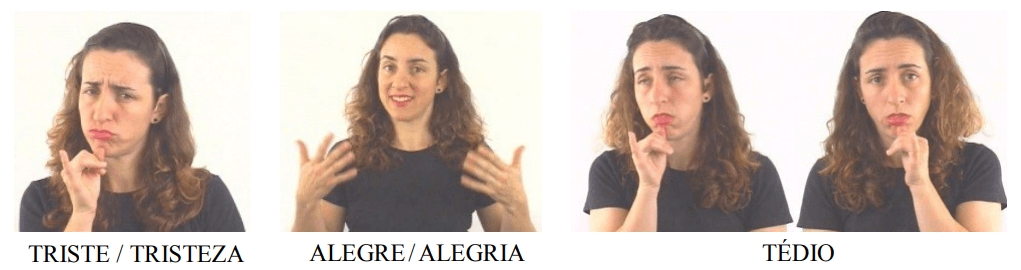
\includegraphics[width=0.8\textwidth]{./figuras/sinaisLibras.png}
    \caption{Parâmetros de formação do sinal na Libras.}
    \label{fig:sinais}
    \fonte{\citeonline{Felipe2013}.}
\end{figure}
 
No nível fonológico, os sinais são formados por parâmetros básicos, conforme detalhado na Figura~\ref{fig:sinais}: a configuração de mão (CM), o movimento (M), a locação (L), a orientação (Or) e as expressões não manuais (ENM). A combinação desses elementos forma os sinais, e mudanças em qualquer um desses parâmetros podem alterar o significado.
 
Do ponto de vista morfológico, a Libras apresenta uma estrutura diferente da língua portuguesa. Em vez de adicionar partes de forma sequencial (como prefixos e sufixos), os elementos do sinal são combinados ao mesmo tempo. Por exemplo, informações como número, negação e até mesmo o objeto da ação podem ser incorporadas diretamente ao sinal. Além disso, a relação entre quem realiza e quem recebe a ação pode ser indicada pela direção do movimento no espaço, utilizando pontos de referência criados durante a comunicação \cite{Quadros2004}.
 
No nível sintático, a língua portuguesa segue predominantemente a ordem Sujeito-Verbo-Objeto (SVO). Já a Libras apresenta maior flexibilidade, sendo possíveis diferentes organizações, como SVO, SOV, OSV e VOS, dependendo do contexto. Isso ocorre porque a língua utiliza o espaço para indicar relações entre os elementos da frase, reduzindo a necessidade de uma ordem fixa. Por exemplo, enquanto em português a sentença "Eu vi o médico" segue obrigatoriamente a ordem sujeito-verbo-objeto, em Libras o objeto pode ser topicalizado e sinalizado antes do verbo, resultando em uma estrutura como MÉDICO EU VER, sem perda de significado \cite{Quadros2004}.
 
Essas diferenças impactam diretamente o processo de tradução automática. Elementos comuns no português, como artigos e preposições, nem sempre aparecem de forma explícita na Libras, pois muitas dessas relações são expressas pelo uso do espaço e pelo contexto.
 
\subsection{Bases de Dados (Datasets)}

No desenvolvimento de modelos de Aprendizado Profundo, o dataset constitui o pilar fundamental para o treinamento e a validação do sistema. Segundo \citeonline{Schmidhuber2014}, a eficácia de arquiteturas como CNNs e LSTMs depende diretamente da disponibilidade de grandes volumes de dados rotulados, que permitem ao modelo aprender representações estatísticas precisas e generalizáveis.

Em problemas que envolvem movimento, uma base de dados robusta deve conter sequências de vídeo que capturem a dinâmica do fenômeno. De acordo com \citeonline{Silva2017}, a diversidade dos dados é crucial para mitigar o sobreajuste (\textit{overfitting}), garantindo que o sistema generalize para diferentes usuários e condições.

Essa diversidade inclui variações antropométricas (tamanho e forma das mãos), condições ambientais (iluminação, fundos complexos) e diferenças na execução (velocidade, amplitude, fluidez). A estruturação do dataset deve prever a divisão entre treinamento, validação e teste, conforme \citeonline{Goodfellow2016}, para avaliar a capacidade de generalização frente a dados nunca vistos.

\subsection{Pré-processamento de Dados}

Antes da aplicação dos modelos, é necessária uma etapa de pré-processamento dos dados visuais para melhorar a qualidade da informação fornecida ao sistema. O pré-processamento envolve redimensionamento dos quadros, normalização dos valores de pixel e remoção de ruídos.

Filtros para suavização e ajuste de contraste reduzem interferências causadas por variações de iluminação e fundo. Segundo \citeonline{Szeliski2010}, essas etapas são fundamentais para que algoritmos de visão computacional extraiam características relevantes de forma eficiente.

A padronização das dimensões e formatos é essencial para o funcionamento correto de redes neurais, especialmente CNNs e LSTMs. Além disso, o balanceamento de classes evita que o modelo favoreça classes majoritárias; estratégias como \textit{data augmentation}, SMOTE e ponderação de classes na função de perda são comuns \cite{Chawla2002, Goodfellow2016}.

\subsection{Visão Computacional}

A Visão Computacional é a ciência que investiga teorias e algoritmos para capacitar sistemas computacionais a emular o sistema visual humano, permitindo que máquinas enxerguem e interpretem o meio à sua volta. 

Por meio da captura de imagens digitais por câmeras e sensores, o sistema extrai, processa e analisa informações significativas que viabilizam o reconhecimento e a manipulação simbólica de objetos \cite{Milano2014}. 

Segundo \citeonline{IBM2025}, enquanto a percepção visual biológica é uma habilidade cognitiva intuitiva e imediata, a visão artificial depende de formulações matemáticas rigorosas para converter matrizes de pixels e dados brutos em conceitos estruturados e representações geométricas tridimensionais.

A metodológia da área abrange desde os níveis mais baixos de processamento até a interpretação semântica de alto nível, englobando a detecção de objetos, o rastreamento de movimento e a modelagem matemática para extração de características. 

No nível básico, procedimentos baseados em matrizes de convolução espacial, como a filtragem digital e as técnicas de redução de ruído Gaussiano ou mediana, operam diretamente no domínio da imagem para ignorar informações espúrias e atenuar frequências irrelevantes do fundo \cite{Milano2014}.

Uma vez suavizado o sinal visual, os métodos avançam para a extração de características latentes, mapeando descontinuidades de intensidade para delinear formas e delimitar trajetórias. 

Na literatura contemporânea, um recurso teórico amplamente adotado é a parametrização por pontos-chave anatômicos (landmarks), que codifica matrizes bidimensionais densas em vetores esparsos de coordenadas espaciais. 

Conforme explicam \citeonline{Pinho2004}, essa decomposição analítica reduz drasticamente a dimensionalidade dos dados brutos, preservando a topologia espacial e as variações cinemáticas que diferenciam as configurações de forma e orientações espaciais dentro de um espaço de busca métrico.

\subsection{MediaPipe e Landmarks}

Os \textit{landmarks} são coordenadas específicas extraídas de partes relevantes do corpo, como articulações das mãos, utilizadas para representar a geometria e o movimento. O MediaPipe é um \textit{framework} de código aberto do Google para construção de \textit{pipelines} de percepção multimodal em tempo real \cite{Lugaresi2019}.

A solução \textit{MediaPipe Hands} opera em dois estágios: um detector localiza a palma da mão produzindo um \textit{bounding box}, e um modelo de regressão estima coordenadas 3D de 21 pontos-chave \cite{Zhang2020}. As coordenadas 
x
x e 
y
y são normalizadas, e 
z
z representa profundidade relativa ao pulso.

Um diferencial do MediaPipe é sua robustez a variações de iluminação e fundo, operando diretamente sobre a imagem bruta \cite{Lugaresi2019}. Sua arquitetura leve atinge taxas superiores a 30 quadros por segundo em hardware convencional, viabilizando aplicações interativas.

\subsection{Deep Learning}

O Aprendizado Profundo (Deep Learning) representa uma evolução conceitual do aprendizado de máquina tradicional, fundamentando-se no paradigma de redes neurais artificiais organizadas em estruturas hierárquicas com múltiplas camadas de processamento não linear.

De acordo com \citeonline{IBM2026}, essa abordagem baseia-se na concepção teórica do córtex visual, simulando redes de processamento onde cada camada subsequente executa transformações matemáticas sobre a saída da camada anterior para aprender representações gradativamente mais abstratas e complexas dos dados textuais ou visuais.

O grande divisor de águas teórico dessa disciplina reside na substituição do desenvolvimento manual de extratores de características (feature engineering) pelo princípio do aprendizado de representações fim-a-fim (end-to-end representation learning), onde o próprio modelo deduz algoritmos matemáticos internos para isolar padrões invariantes a partir dos dados em sua forma mais bruta \cite{Oracle2022}.

Esse mecanismo de autoajuste é governado pelo ajuste dinâmico de tensores de pesos e vieses através de algoritmos de retropropagação do erro acoplados à descida de gradiente estocástica, conferindo às redes profundas a propriedade matemática de aproximadores universais \cite{Goodfellow2016}.

Segundo \citeonline{Schmidhuber2014}, o advento do aprendizado profundo causou uma ruptura no reconhecimento de padrões ao fornecer formulações matemáticas capazes de modelar dependências estruturais de alta dimensionalidade em grandes volumes de dados não estruturados.

Desse modo, o arcabouço teórico do Deep Learning fundamenta-se na capacidade de projetar espaços latentes onde entradas massivas e altamente não lineares são projetadas em variedades topológicas simples, permitindo classificações e mapeamentos de extrema precisão matemática \cite{Goodfellow2016}.

\subsection{Redes Neurais Convolucionais (CNN)}

As Redes Neurais Convolucionais são arquiteturas especializadas no processamento de dados com topologia em grade, como imagens. Introduzidas por \citeonline{Lecun1998} e popularizadas com o AlexNet \cite{Krizhevsky2012}, elas substituem a extração manual de características por aprendizado hierárquico.

A arquitetura inclui camadas de convolução, onde filtros deslizam sobre a entrada calculando o produto escalar, gerando mapas de ativação. O compartilhamento de pesos confere invariância à translação \cite{Goodfellow2016}. As camadas de \textit{pooling} realizam subamostragem espacial, reduzindo parâmetros e custo computacional \cite{Lecun1998}.

Ao final, camadas totalmente conectadas combinam as representações abstratas para gerar a predição final \cite{Furtado2019}. As CNNs aprendem características de forma hierárquica: bordas e texturas nas camadas iniciais, objetos completos nas mais profundas \cite{Fleck2016}.

\subsection{Redes de Memória de Longo Prazo (LSTM)}

A Long Short-Term Memory (LSTM) é uma arquitetura recorrente introduzida por \citeonline{Hochreiter1997} para resolver o problema do desaparecimento do gradiente, que impede redes comuns de aprender dependências de longo prazo em sequências.

O diferencial da LSTM é sua unidade de memória interna (célula), que mantém informações por intervalos estendidos \cite{Hochreiter1997}. Três portões controlam o fluxo: o portão de esquecimento descarta informações antigas, o portão de entrada armazena novas informações, e o portão de saída determina o que será enviado ao próximo passo \cite{Contarini2020}.

Segundo \citeonline{Schmidhuber2014}, a profundidade temporal dessas redes possibilita a extração de representações abstratas que conectam sequências de entradas a conceitos semânticos complexos. As LSTMs são fundamentais para tarefas onde a classificação depende de eventos ocorridos muitos passos atrás.

\subsection{Reconhecimento de Gestos (\textit{Gesture Recognition})}

O reconhecimento de gestos constitui uma vertente altamente especializada da visão computacional dedicada ao mapeamento, modelagem e categorização de posturas, movimentos e orientações cinemáticas do corpo humano a partir de fluxos contínuos de dados visuais \cite{Silva2017}.

Do ponto de vista puramente conceitual, as manifestações gestuais humanas são divididas formalmente pela literatura em duas grandes classes operacionais, cujas propriedades matemáticas exigem formulações algorítmicas de naturezas distintas:

Gestos Estáticos: São definidos teoricamente como configurações espaciais discretas que independem do fator temporal, cuja informação semântica está inteiramente contida em uma única amostra de imagem. O foco analítico recai sobre as propriedades de forma, orientação angular e posicionamento relativo dos segmentos anatômicos, características cuja modelagem é tratada com eficiência por meio de operadores de convolução espacial capazes de extrair invariâncias geométricas locais \cite{PintoJunior2019}.

Gestos Dinâmicos: São definidos como trajetórias espaço-temporais contínuas onde o significado da ação está intrinsecamente codificado na evolução do movimento ao longo do eixo do tempo. Diferente da classe estática, os gestos dinâmicos são modelados por funções de velocidade, aceleração e deslocamento, exigindo estruturas algébricas e redes recorrentes capazes de computar dependências sequenciais e continuidade temporal a partir de matrizes residuais ou diferenciais de quadros adjacentes \cite{Monteiro2016}.

A formalização teórica desses sistemas impõe o enfrentamento de severas fontes de ruído matemático que afetam a robustez dos modelos de classificação. O primeiro grande desafio conceitual decorre das variações de iluminação, fenômeno que altera a função de reflectância da cena e modifica drasticamente os valores dos pixels, inserindo ruídos não lineares que dificultam a segmentação e a extração correta de histogramas ou gradientes de pele \cite{Bittencourt2002}.

O segundo fator diz respeito à variabilidade morfométrica e comportamental entre usuários, visto que diferentes indivíduos executam o mesmo padrão gestual com amplitudes e velocidades distintas sob geometrias manuais variadas, o que exige a formulação de espaços de características dotados de propriedades de alta generalização \cite{Silva2017}.

Por fim, a complexidade inerente ao plano de fundo (background clutter) introduz oclusões e texturas concorrentes que compartilham propriedades cromáticas ou espaciais com o objeto de interesse, demandando o desenvolvimento de filtros adaptativos e técnicas de isolamento topológico para garantir que a atenção algorítmica permaneça concentrada estritamente na estrutura gestual analisada \cite{Bittencourt2002, Silva2017}.

\subsection{Processamento de Linguagem Natural (NLP)}

O Processamento de Linguagem Natural (NLP) capacita sistemas a compreender, interpretar e gerar a linguagem humana em formato de texto. Segundo \citeonline{Stryker2024}, o NLP combina linguística computacional com aprendizado profundo para processar a linguagem com compreensão de significado e intenção.

Tarefas fundamentais incluem tokenização (divisão em unidades lexicais), etiquetagem morfossintática (classificação de tokens como substantivos, verbos etc.), análise de dependência sintática e geração de linguagem natural. Conforme \citeonline{Lopez2017}, redes neurais aplicadas ao NLP lidam com a ambiguidade e aprendem representações hierárquicas dos dados textuais.

\subsection{Árvores de Dependência Sintática}

Uma árvore de dependência sintática representa as relações gramaticais binárias entre os tokens de uma sentença. Diferentemente de gramáticas de constituintes, a análise de dependência conecta diretamente pares de palavra-cabeça e dependente, com etiquetas como \textit{nsubj} (sujeito) ou \textit{obj} (objeto) \cite{Jurafsky2023}.

Formalmente, cada token (exceto a raiz) possui exatamente uma cabeça, garantindo a estrutura de árvore \cite{Jurafsky2023}. Essa abordagem é adequada para línguas com ordem frasal flexível, pois identifica relações semânticas independentemente da posição linear dos tokens.

As etiquetas de dependência permitem aplicar regras de concordância dirigidas: identificado o sujeito, é possível flexionar o verbo-cabeça no número e pessoa correspondentes \cite{Bird2009}.

\subsection{Modelos de Linguagem de Grande Escala (LLM)}

Os Modelos de Linguagem de Grande Escala (LLMs) são sistemas treinados em vastos volumes de dados textuais, baseados na arquitetura Transformer \cite{Vaswani2017}. Eles utilizam mecanismos de auto-atenção para capturar dependências de longo alcance de forma paralela.

LLMs apresentam capacidade de \textit{few-shot learning}: com poucos exemplos no contexto, realizam novas tarefas sem atualização dos pesos \cite{Brown2020}. Modelos como Llama \cite{Touvron2023} e Gemma \cite{GemmaTeam2024} são de código aberto e podem ser executados localmente.

Esses modelos aprendem padrões estatísticos sofisticados da linguagem, corrigindo ambiguidades, inserindo elementos implícitos e ajustando o registro formal ou informal de sentenças.

\subsection{Métricas: Acurácia, Matriz de Confusão e BLEU}

A acurácia expressa a proporção de predições corretas em relação ao total de exemplos, sendo a métrica mais fundamental para classificação \cite{Goodfellow2016}. No entanto, ela pode ser insuficiente em problemas com muitas classes ou desbalanceamento.

A matriz de confusão é uma tabela que cruza classes reais com classes preditas, permitindo identificar padrões de erro específicos. A partir dela derivam-se precisão e \textit{recall}, métricas que expõem desequilíbrios de desempenho \cite{Goodfellow2016}.

Para avaliação de tradução, o BLEU (\textit{Bilingual Evaluation Understudy}) compara o texto gerado com referências humanas, medindo a sobreposição de n-gramas. Unigramas avaliam palavras isoladas; bigramas e trigramas verificam ordem e contexto. O escore BLEU varia de 0 a 1 e penaliza desvios estruturais \cite{Papineni2002}.

\subsection{Latência e Tempo de Resposta}

A latência corresponde ao tempo decorrido entre a entrada de um dado no sistema e a produção da resposta correspondente. Em aplicações interativas em tempo real, a latência impacta diretamente a experiência do usuário e a fluidez da comunicação.

Sistemas com alta latência geram atrasos perceptíveis, comprometendo a interação. Segundo \citeonline{Molchanov2015}, em sistemas de reconhecimento de gestos em tempo real, o desempenho está ligado à eficiência computacional dos modelos e à sua capacidade de processar sequências com baixa latência.

Reduzir a latência exige otimização de todo o \textit{pipeline}: captura, pré-processamento, inferência e geração de saída. Em hardware convencional, busca-se um equilíbrio entre precisão, consumo energético e tempo de resposta.

\subsection{Custo Computacional e Peso dos Modelos}

O custo computacional refere-se aos recursos necessários para executar um modelo, incluindo memória, processamento e armazenamento. O peso do modelo está relacionado ao número de parâmetros treináveis, influenciando diretamente seu tamanho e complexidade.

Modelos mais complexos tendem a apresentar maior precisão, porém demandam mais recursos. Conforme \citeonline{Goodfellow2016}, o aumento da profundidade eleva a capacidade de representação, mas implica maior custo e necessidade de hardware robusto.

Em sistemas de tempo real, é essencial equilibrar precisão e eficiência para operar com baixa latência em hardware convencional. Técnicas de compressão como poda e quantização ajudam a reduzir o peso dos modelos sem degradação severa da acurácia.


% ---------------------------------------------------------------
\section{Metodologia da pesquisa bibliográfica}
\label{sec:metodologia_pesquisa}

A pesquisa bibliográfica foi realizada nas bases Google Scholar e IEEE Xplore, utilizando as strings de busca "Libras" AND "Deep Learning" AND "Visão Computacional", "Reconhecimento de sinais" AND "Libras" AND ("CNN" OR "LSTM") e "Língua Brasileira de Sinais" AND "Acessibilidade" AND "Redes Neurais". Foram selecionados artigos publicados entre 2021 e 2026, em português e inglês, que abordassem diretamente o reconhecimento automático de sinais, técnicas de visão computacional aplicadas à Libras e métodos de processamento de linguagem natural voltados à tradução de linguagem de sinais.

% \textit{} italico

% ---------------------------------------------------------------
\section{Fundamentos}
\label{sec:fundamentos}

Esta seção detalha como os conceitos apresentados no Referencial Teórico são aplicados concretamente na construção do sistema proposto. A organização segue o fluxo do \textit{pipeline} de tradução: da coleta e preparação dos dados ao reconhecimento dos gestos, ao pós-processamento linguístico e, por fim, à avaliação do desempenho.
 
% --- GRUPO 1 ---
\subsection{Grupo 1: Coleta de Dados e Tratamentos}
 
Este grupo descreve como os dados de Libras são selecionados, organizados e preparados para o treinamento do sistema, envolvendo a escolha dos datasets, as estratégias de pré-processamento e a extração de \textit{landmarks} pelo MediaPipe.
 
\subsubsection{Datasets}
 
Os três datasets adotados neste projeto foram selecionados pela diversidade de sinalizadores, vocabulário e modalidade de captura. O MINDS-Libras \cite{Rezende2021} conta com distribuição controlada: 6 pessoas realizando 5 repetições de cada um dos 20 sinais, resultando em classes uniformes. O V-Librasil \cite{Rodrigues2021} possui estrutura igualmente regular, com exatamente 3 gravações por sinal para cada um dos 1.364 termos. Já o Libras Brazilian Sign Language \cite{Pas2020}, composto por imagens estáticas do alfabeto manual, apresenta variação relevante no número de amostras entre as classes.
 
A integração dos três datasets pode ampliar desequilíbrios, visto que as interseções de vocabulário entre eles são parciais e as quantidades de amostras por sinal diferem. Para compor um conjunto de treinamento robusto, cada base contribui com uma cobertura distinta: o MINDS-Libras e o V-Librasil cobrem sinais dinâmicos com contexto de múltiplos sinalizadores, enquanto o Libras Brazilian Sign Language oferece ampla variedade de configurações estáticas do alfabeto manual.
 
\subsubsection{Pré-processamento de Dados}
 
O pré-processamento dos dados neste projeto inclui etapas de tratamento de imagem e de balanceamento de classes. Para o tratamento visual, são aplicados redimensionamento dos \textit{frames}, normalização dos valores de pixel e remoção de ruídos, garantindo que todas as sequências e imagens possuam dimensões e formatos consistentes como entrada para os modelos CNN e LSTM \cite{Szeliski2010}.
 
Para mitigar o desequilíbrio entre classes decorrente da integração dos três datasets, serão adotadas estratégias complementares: \textit{data augmentation} (espelhamento, rotações e variações de velocidade dos vídeos) para aumentar as classes minoritárias; SMOTE (\textit{Synthetic Minority Over-sampling Technique}), aplicado sobre os vetores de \textit{landmarks} extraídos pelo MediaPipe — e não diretamente sobre pixels —, gerando exemplos sintéticos por interpolação entre amostras próximas no espaço de características \cite{Chawla2002}; e ponderação de classes na função de perda durante o treinamento, penalizando mais os erros cometidos nas classes menos frequentes \cite{Goodfellow2016}.
 
O pré-processamento também inclui a preparação das sequências de vídeo para o modelo LSTM, organizando os \textit{frames} de forma temporal. Para os sinais estáticos destinados à CNN, cada imagem é individualmente normalizada e redimensionada para garantir uniformidade de entrada.
 
\subsubsection{MediaPipe e Landmarks}
 
No contexto deste projeto, o MediaPipe Hands substitui o processamento direto sobre pixels das imagens de câmera. Em vez de alimentar os modelos CNN e LSTM com \textit{frames} completos — o que elevaria o custo computacional e aumentaria a sensibilidade a ruídos visuais —, o sistema extrai os 21 \textit{landmarks} por mão (totalizando até 63 coordenadas por \textit{frame} quando duas mãos estão presentes) e utiliza esses vetores compactos como representação de entrada. Essa escolha reduz drasticamente a dimensionalidade dos dados, acelera o treinamento e a inferência, e torna o sistema mais generalizável entre diferentes usuários, pois a representação baseada em articulações é invariante a variações de tom de pele e textura das mãos \cite{Lugaresi2019}.
 
O SMOTE, mencionado na etapa de pré-processamento, é aplicado diretamente sobre esses vetores de \textit{landmarks} — e não sobre os \textit{frames} brutos —, o que garante que a augmentação sintética preserve a estrutura geométrica dos sinais, sem introduzir artefatos visuais \cite{Chawla2002}.
 
% --- GRUPO 2 ---
\subsection{Grupo 2: Leitura dos Gestos}
 
Este grupo descreve como o sistema interpreta os dados de \textit{landmarks} para reconhecer sinais de Libras, combinando arquiteturas de visão computacional e aprendizado profundo para tratar tanto sinais estáticos quanto dinâmicos.
 
\subsubsection{Visão Computacional Aplicada à Detecção de Mãos}
 
No desenvolvimento deste projeto, a aplicação da visão computacional concentra-se prioritariamente na detecção de mãos. Essa etapa é crucial para localizar e isolar os membros superiores do restante do cenário, garantindo que os \textit{landmarks} extraídos pelo MediaPipe representem exclusivamente a configuração dos sinais \cite{Neves2012}. O sistema descarta \textit{frames} em que nenhuma mão for detectada, evitando a inserção de ruído no processo de reconhecimento.
 
\subsubsection{Deep Learning: CNN e LSTM}
 
O uso do \textit{deep learning} neste projeto justifica-se pela necessidade de tratar informações visuais e sequenciais simultaneamente. Redes profundas são aproximadores universais capazes de mapear entradas complexas para saídas específicas \cite{Goodfellow2016}, o que permite ao sistema aprender, a partir dos vetores de \textit{landmarks}, as combinações de posições articulares que caracterizam cada sinal.
 
Para sinais estáticos, como as configurações de mão do alfabeto manual da Libras, é empregada uma CNN. Os \textit{landmarks} extraídos pelo MediaPipe (coordenadas $x$, $y$, $z$ das articulações) são organizados como vetores de entrada para a rede, que aprende, durante o treinamento, quais combinações de posições articulares são discriminativas para cada sinal. As camadas iniciais capturam padrões simples (orientação dos dedos, curvatura das juntas) e as camadas mais profundas combinam esses padrões em representações de alto nível (configuração completa da mão) \cite{Fleck2016}.
 
Para sinais dinâmicos, cuja compreensão depende da trajetória e da sequência de movimentos ao longo do tempo, utiliza-se a LSTM. Cada \textit{frame} capturado pela câmera contribui com um vetor de \textit{landmarks}, e a LSTM processa essa sequência temporal de vetores para identificar o sinal. A capacidade de retenção temporal da LSTM permite que o sistema compreenda que a trajetória e a transição entre as poses das mãos são tão importantes quanto a configuração isolada em um único \textit{frame} \cite{Almeida2019}.
 
\begin{figure}[H]
    \centering
    
\includegraphics[width=0.8\textwidth]{./figuras/lstm}
    \caption{Diagrama de Rede Neural LSTM.}
    \source{Autoria própria (2026).}
\end{figure}
 
\subsubsection{Reconhecimento de Gestos no Pipeline}
 
A arquitetura híbrida CNN+LSTM cobre as duas categorias de gestos presentes na Libras: estáticos e dinâmicos. Após a detecção das mãos pelo MediaPipe, o sistema identifica o tipo de sinal e encaminha os dados para o modelo correspondente. O resultado de ambas as arquiteturas é um token — uma palavra ou conceito reconhecido —, que é então encaminhado para a fila de entrada do módulo de NLP.
 
Os principais desafios enfrentados nesta etapa incluem a variabilidade entre usuários (diferenças físicas, velocidade e amplitude de execução) e a dependência de um vocabulário inicial delimitado, necessária para garantir o rigor técnico do sistema neste estágio experimental \cite{Silva2017}.
 
% --- GRUPO 3 ---
\subsection{Grupo 3: Pós-processamento Linguístico}
 
Este grupo descreve como os tokens reconhecidos pelo módulo de visão computacional são transformados em frases gramaticalmente corretas em português, por meio de um \textit{pipeline} de NLP implementado com spaCy e refinado por um LLM.
 
\subsubsection{Módulo de NLP com spaCy}
 
O reconhecimento isolado de gestos não é suficiente para uma comunicação fluida, dada a profunda divergência gramatical entre a Libras e a língua portuguesa. O módulo de NLP atua como uma camada de pós-processamento essencial, realizando a conversão semântica e sintática dos sinais identificados pela rede neural.
 
A abordagem adotada é um \textit{pipeline} de processamento sequencial, implementado com a biblioteca spaCy \cite{Honnibal2020}, composto por quatro etapas:
 
\begin{enumerate}
    \item \textbf{Tokenização e normalização:} os sinais identificados chegam ao módulo como uma sequência de tokens na estrutura da Libras (ex.: \texttt{[VOCÊ, QUERER, ÁGUA]}). Cada sinal é tratado como uma unidade lexical discreta, e a lematização reduz as formas flexionadas à forma canônica, facilitando o mapeamento para o português \cite{Bird2009};
    \item \textbf{Etiquetagem morfossintática:} cada token recebe uma etiqueta (substantivo, verbo, pronome, etc.), por meio de um modelo de rede neural treinado sobre corpora anotados \cite{Honnibal2020};
    \item \textbf{Análise de dependência sintática:} o analisador identifica as relações gramaticais entre os tokens (sujeito, objeto, modificador, etc.), produzindo uma árvore de dependência sintática. A adoção de árvores de dependência é especialmente adequada para a Libras porque a análise de dependência é robusta a variações de ordem frasal, identificando as relações semânticas independentemente da posição linear dos tokens \cite{Jurafsky2023};
    \item \textbf{Reordenação sintática e concordância:} com base nas relações da árvore de dependência, o módulo reordena os tokens segundo a estrutura SVO do português e aplica regras de concordância nominal e verbal. Por exemplo, a sequência \texttt{[VOCÊ, QUERER, ÁGUA]} é reescrita como \textit{``Você quer água.''}, com a flexão verbal adequada ao sujeito identificado \cite{Lopez2017}.
\end{enumerate}
 
Formalmente, seja $S_L = (w_1, w_2, \ldots, w_n)$ a sequência de sinais na estrutura da Libras e $S_P$ a frase-alvo em português. O módulo aprende uma função de reordenação $\pi$ tal que:
 
\begin{equation}
    S_P = \text{Flexão}\bigl(\pi(S_L),\; G_{\text{pt}}\bigr)
\end{equation}
 
onde $\pi$ é uma permutação dos índices dos tokens guiada pelas relações de dependência e $G_{\text{pt}}$ representa as regras gramaticais do português, incluindo concordância de gênero, número e tempo verbal \cite{Bird2009}.
 
\begin{figure}[H]
    \centering
    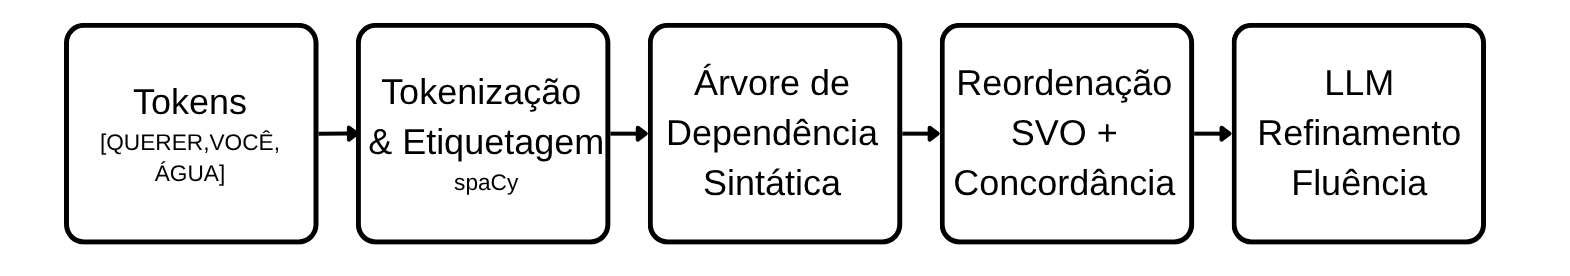
\includegraphics[width=0.4\textwidth]{./figuras/processamento-de-imagem-nlp}
    \caption{Diagrama de Processamento de Linguagem Natural - NLP.}
    \source{Autoria própria (2026).}
\end{figure}
 
\subsubsection{Refinamento via LLM}
 
No fluxo de tradução proposto, o LLM atua como uma camada de refinamento linguístico final. Após o módulo de NLP (spaCy) organizar a estrutura sintática básica e realizar as flexões necessárias, o LLM recebe essa sentença intermediária para otimizar sua naturalidade. Essa etapa é essencial para ajustar nuances que as regras gramaticais determinísticas podem não captar, como a inserção de conectivos contextuais, artigos ou preposições ausentes, e o ajuste de registro (formal ou informal), garantindo que a saída em português não seja apenas gramaticalmente correta, mas também fluida \cite{Brown2020}.
 
A integração de modelos como Llama \cite{Touvron2023} ou Gemma \cite{GemmaTeam2024} permite que o sistema aproveite a capacidade de \textit{few-shot learning}, refinando traduções a partir de poucos exemplos de contexto, sem a necessidade de um novo treinamento exaustivo.
 
% --- GRUPO 4 ---
\subsection{Grupo 4: Métricas e Validação}
 
Este grupo descreve como o desempenho do sistema será mensurado, abrangendo tanto a avaliação do módulo de reconhecimento gestual quanto a qualidade linguística das traduções e a viabilidade de uso em tempo real.
 
\subsubsection{Acurácia e Matriz de Confusão}
 
No escopo desta pesquisa, a acurácia e a matriz de confusão serão utilizadas para avaliar o módulo de visão computacional, tanto na classificação de sinais estáticos pela CNN quanto no reconhecimento de sinais dinâmicos pela LSTM. A análise conjunta dessas métricas permitirá identificar os sinais com maior taxa de erro — por exemplo, pares de sinais que o modelo tende a confundir devido à semelhança na configuração de mão ou no movimento — e orientar ajustes no modelo ou na composição do dataset de treinamento \cite{Goodfellow2016}. Com essa abordagem, busca-se garantir que o sistema apresente desempenho equilibrado entre todos os sinais do vocabulário definido, e não apenas nas classes mais frequentes.
 
\subsubsection{Métrica BLEU}
 
O uso do BLEU é especialmente relevante neste projeto porque o módulo de NLP não apenas transcreve sinais isolados, mas reorganiza e flexiona as palavras para gerar frases coerentes em português — um processo que não pode ser avaliado somente por acurácia. Para a validação do sistema, o BLEU será calculado comparando as frases em português produzidas pelo sistema com traduções de referência elaboradas por especialistas para o mesmo conjunto de sinais de entrada. Escores mais altos indicarão que o módulo de NLP está gerando saídas linguisticamente próximas ao que um humano produziria a partir dos mesmos sinais. Nesse sentido, o BLEU complementa as métricas de reconhecimento gestual ao avaliar especificamente a qualidade da camada linguística, fechando o ciclo de avaliação do \textit{pipeline} completo \cite{Papineni2002}.
 
\subsubsection{Custo Computacional e Latência}
 
No contexto deste projeto, a escolha das arquiteturas busca equilibrar desempenho e eficiência, considerando a necessidade de processamento em tempo de execução. A utilização de \textit{landmarks} como representação de entrada — em vez de \textit{frames} completos — reduz drasticamente a dimensionalidade dos dados, diminuindo o custo de treinamento e inferência. A limitação do vocabulário inicial também contribui para manter os modelos dentro de um tamanho viável para execução em hardware convencional.
 
A latência será considerada como um dos principais critérios de avaliação do sistema. Serão medidos os tempos de cada etapa do \textit{pipeline} — captura de vídeo, extração de \textit{landmarks}, inferência CNN ou LSTM, processamento NLP e refinamento LLM — para identificar gargalos e verificar se o sistema é viável para uso em tempo real. Conforme apontado por \citeonline{Molchanov2015}, em sistemas de reconhecimento de gestos, o desempenho está diretamente relacionado à eficiência computacional dos modelos e à capacidade de processar sequências de vídeo com baixa latência.
 
% --- GRUPO 5 ---
\subsection{Grupo 5: Integração do Pipeline}
 
Os grupos descritos anteriormente não operam de forma isolada: eles se articulam em um \textit{pipeline} sequencial que transforma o fluxo de vídeo capturado pela câmera em uma frase coerente em português. Esta seção descreve como essas etapas se conectam e os desafios específicos dessa integração.
 
O fluxo começa com a captura contínua de \textit{frames} pela webcam. Para cada \textit{frame}, o MediaPipe tenta detectar a presença de mãos. Se mãos forem detectadas, os 21 \textit{landmarks} por mão são extraídos e normalizados (Grupo 1). O vetor de \textit{landmarks} resultante é então encaminhado para o módulo de classificação: se o sinal for estático, a CNN processa o vetor e emite um token; se for dinâmico, a LSTM acumula vetores ao longo de uma janela temporal e emite o token ao identificar o sinal completo (Grupo 2). Os tokens reconhecidos são enfileirados até que um critério de fim de sentença seja satisfeito (pausa ou sinal explícito). Nesse ponto, a sequência de tokens é entregue ao módulo de NLP (spaCy), que realiza a reordenação sintática e as flexões necessárias (Grupo 3). A frase resultante é então enviada ao LLM para refinamento linguístico final, e o texto fluente em português é exibido na interface do usuário (Grupo 3). Por fim, as métricas de avaliação são coletadas ao longo de sessões de teste para validar o desempenho do sistema (Grupo 4).
 
Um dos principais desafios dessa integração está na necessidade de sincronizar os diferentes tempos de processamento de cada etapa. O MediaPipe opera em tempo real a mais de 30 \textit{frames} por segundo, enquanto a inferência da LSTM exige o acúmulo de uma sequência mínima de \textit{frames}, e o LLM introduz latência adicional no refinamento da sentença. Para garantir fluidez, o \textit{pipeline} é projetado com filas assíncronas entre os módulos, de modo que a captura de vídeo não seja bloqueada pelo processamento linguístico.
 
Outro desafio é a fronteira entre sinais: o sistema precisa identificar quando um gesto termina e o próximo começa, especialmente para sinais dinâmicos com movimentos similares nas fases de transição. Essa detecção de segmentação temporal é tratada por um limiar de confiança nas saídas da LSTM: tokens com confiança abaixo de um valor definido são descartados e exibem um alerta na interface, evitando que erros de reconhecimento contaminem a sentença gerada.

% ---------------------------------------------------------------
\section{Trabalhos relacionados}
\label{sec:trabalhos_relacionados}

\subsection{Trabalho 1: Sign Language Translator System Using Computer Vision and LSTM Neural Networks}

O estudo de \citeonline{Wang2025} investigou o problema da dificuldade de comunicação entre pessoas surdas e ouvintes, causada pela falta de compreensão da língua de sinais, o que impacta diretamente o acesso a serviços e interações sociais — o mesmo problema abordado neste trabalho.

Para enfrentar essa questão, os autores desenvolveram um sistema de tradução de língua de sinais em tempo real, combinando técnicas de visão computacional, redes neurais convolucionais (CNN), redes recorrentes do tipo LSTM e processamento de linguagem natural. A metodologia incluiu a coleta e anotação de um dataset de gestos, seguido do treinamento de modelos capazes de reconhecer sinais e convertê-los em texto automaticamente.

Os resultados obtidos demonstraram uma precisão de 97\% no reconhecimento dos gestos, indicando que a abordagem é eficaz para cenários controlados. Além disso, o sistema mostrou potencial para melhorar a acessibilidade e a inclusão social.

Entretanto, a solução apresenta limitações importantes, como a dependência de condições ambientais controladas (iluminação e fundo), a escassez de datasets amplos, e dificuldades em manter desempenho em tempo real. Também há restrições relacionadas à acessibilidade, especialmente em sistemas baseados na web que dependem de conexão com a internet.

Diferentemente desse trabalho, a presente pesquisa propõe uma abordagem mais integrada, ao não apenas reconhecer os sinais, mas também estruturá-los linguisticamente por meio de processamento de linguagem natural, buscando gerar frases coerentes em português, e não apenas transcrições diretas de sinais.

\subsection{Trabalho 2: Interpretação de gestos de Libras usando K-Means e Random Forest}

\citeonline{Caiafa2023} propuseram uma solução para o reconhecimento automático de sinais da Libras com foco em reduzir o custo computacional, mantendo uma boa acurácia. O problema tratado também está relacionado à barreira de comunicação entre usuários e não usuários da língua de sinais, sendo, portanto, diretamente alinhado com esta pesquisa.

A abordagem adotada pelos autores difere das soluções baseadas exclusivamente em \textit{deep learning}, pois utiliza o MediaPipe para extração de pontos-chave corporais, seguido de técnicas de agrupamento com K-Means e classificação utilizando algoritmos como KNN e Random Forest. Essa metodologia permite trabalhar com representações mais leves dos dados, reduzindo o processamento necessário.

Os experimentos foram realizados utilizando a base de dados MINDS-Libras, resultando em uma acurácia de 94,72\%, demonstrando que a solução é eficiente mesmo com menor complexidade computacional.

Apesar dos bons resultados, o trabalho apresenta limitações, principalmente no fato de que o sistema foca apenas na classificação de sinais isolados, sem tratar a construção de frases ou o contexto linguístico. Além disso, ainda enfrenta desafios comuns da área, como variações de iluminação, ângulo de câmera e aumento do vocabulário.

O presente trabalho avança em relação a essa proposta ao incorporar, além da etapa de reconhecimento, um módulo de processamento de linguagem natural, responsável por organizar os sinais identificados em frases estruturadas em português, ampliando o nível de interpretação da comunicação.

\subsection{Trabalho 3: Detection and Interpretation of Indian Sign Language Using LSTM Networks}

\citeonline{Vyavahare2023} abordaram o desenvolvimento de um sistema para reconhecimento e interpretação da língua de sinais indiana (ISL) em tempo real, com o objetivo de reduzir a lacuna comunicacional entre pessoas com deficiência auditiva e a sociedade — problema equivalente ao tratado neste TCC.

A solução proposta baseia-se no uso de técnicas de visão computacional para extração de características visuais, combinadas com redes neurais recorrentes do tipo LSTM, capazes de capturar dependências temporais em gestos dinâmicos. Os autores também criaram um dataset próprio, composto por vídeos anotados de usuários nativos de ISL.

Os resultados experimentais indicaram um desempenho elevado, com 96% de acurácia no treinamento e 87% no teste, evidenciando a capacidade do modelo em reconhecer padrões gestuais dinâmicos.

No entanto, o estudo apresenta algumas limitações relevantes. A principal delas é que o sistema está restrito ao reconhecimento de palavras isoladas, não sendo capaz de interpretar frases completas. Além disso, o desempenho pode ser afetado por fatores como variações de iluminação, ângulo de câmera e posicionamento das mãos.

Este trabalho se diferencia ao propor uma solução que vai além do reconhecimento de gestos individuais, incorporando uma camada de processamento de linguagem natural para construção de frases, buscando uma tradução mais próxima da comunicação real entre Libras e língua portuguesa.

\vspace{0.5cm}

\begin{table}[htb]
    \centering
    \caption{Comparação entre trabalhos relacionados}
    \label{tab:trabalhos_relacionados}
    \small % Reduz levemente o tamanho da fonte para caber melhor na página
    \begin{tabular}{p{2cm}|p{3cm}|p{3cm}|p{3cm}|p{3cm}}
        \toprule
        \textbf{Critério} & \textbf{Trabalho 1} & \textbf{Trabalho 2} & \textbf{Trabalho 3} & \textbf{Este trabalho} \\
        \midrule
        \textbf{Objetivo} 
        & Tradução de sinais em tempo real para texto. 
        & Classificação de sinais de Libras com baixo custo computacional. 
        & Reconhecimento e interpretação de sinais dinâmicos (ISL). 
        & Tradução de Libras com estruturação gramatical de frases. \\
        \midrule
        \textbf{Tecnologia} 
        & CNN, LSTM e PLN básico. 
        & MediaPipe, K-Means, KNN e Random Forest. 
        & Visão Computacional (OpenCV) e LSTM. 
        & Arquitetura híbrida CNN + LSTM e camada robusta de PLN. \\
        \midrule
        \textbf{Validação} 
        & Dataset próprio (webcam); Acurácia de 97\%. 
        & Base pública MINDS-Libras; Acurácia de 94,72\%. 
        & Dataset próprio (ISL); 96\% treino e 87\% teste. 
        & Dataset de Libras, métricas de acurácia e avaliação sintática. \\
        \midrule
        \textbf{Limitação} 
        & Sensível à iluminação e dependência de conexão web. 
        & Classificação restrita a sinais/palavras isoladas. 
        & Não interpreta frases completas ou contexto linguístico. 
        & Dependência de dataset abrangente para diversidade de sinais. \\
        \bottomrule
    \end{tabular}
    \\
    \source{Autoria própria (2026).}
\end{table}

% ===============================================================
% CAPÍTULO 3 - DESENVOLVIMENTO
% ===============================================================
\chapter{Desenvolvimento}
\label{cap:desenvolvimento}

Neste capítulo, apresenta-se a solução proposta para o problema de tradução automática da Língua Brasileira de Sinais (Libras) para a língua portuguesa. A descrição contempla a visão geral do sistema, sua arquitetura, as tecnologias selecionadas, as funcionalidades principais, a metodologia de desenvolvimento adotada e os critérios de validação que serão utilizados para avaliar o desempenho da solução.

\begin{figure}[H]
    \centering
    
\includegraphics[width=0.6\textwidth]{./figuras/arquitetura-sistema}
    \caption{Diagrama de fluxo da solução proposta.}
    \source{Autoria própria (2026).}
\end{figure}

% ---------------------------------------------------------------
\section{Solução proposta}
\label{sec:solucao}

\subsection{Visão geral da solução}
A solução proposta consiste em um sistema desktop de tradução automática em tempo execução, capaz de reconhecer gestos da Língua Brasileira de Sinais por meio de visão computacional e convertê-los em texto da língua portuguesa. O sistema é voltado para uso em computadores com câmera integrada, sendo projetado para funcionar como um facilitador de comunicação em contextos como atendimentos, ambientes educacionais e interações cotidianas.

A aplicação é composta por três módulos principais integrados em um pipeline de processamento sequencial: (i) o módulo de visão computacional, responsável pela captura e reconhecimento dos sinais; (ii) o módulo de processamento de linguagem natural, responsável pela conversão dos tokens reconhecidos em frases coerentes em português; e (iii) a interface do usuário, que exibe a tradução em tempo execução.

Em razão da amplitude lexical da Libras e do caráter experimental deste estudo, o vocabulário inicial do sistema abrangerá um conjunto definido de sinais voltados a contextos de comunicação básica, como cumprimentos, solicitações de ajuda, identificação pessoal e situações de atendimento.
\begin{figure}[H]
    \centering
    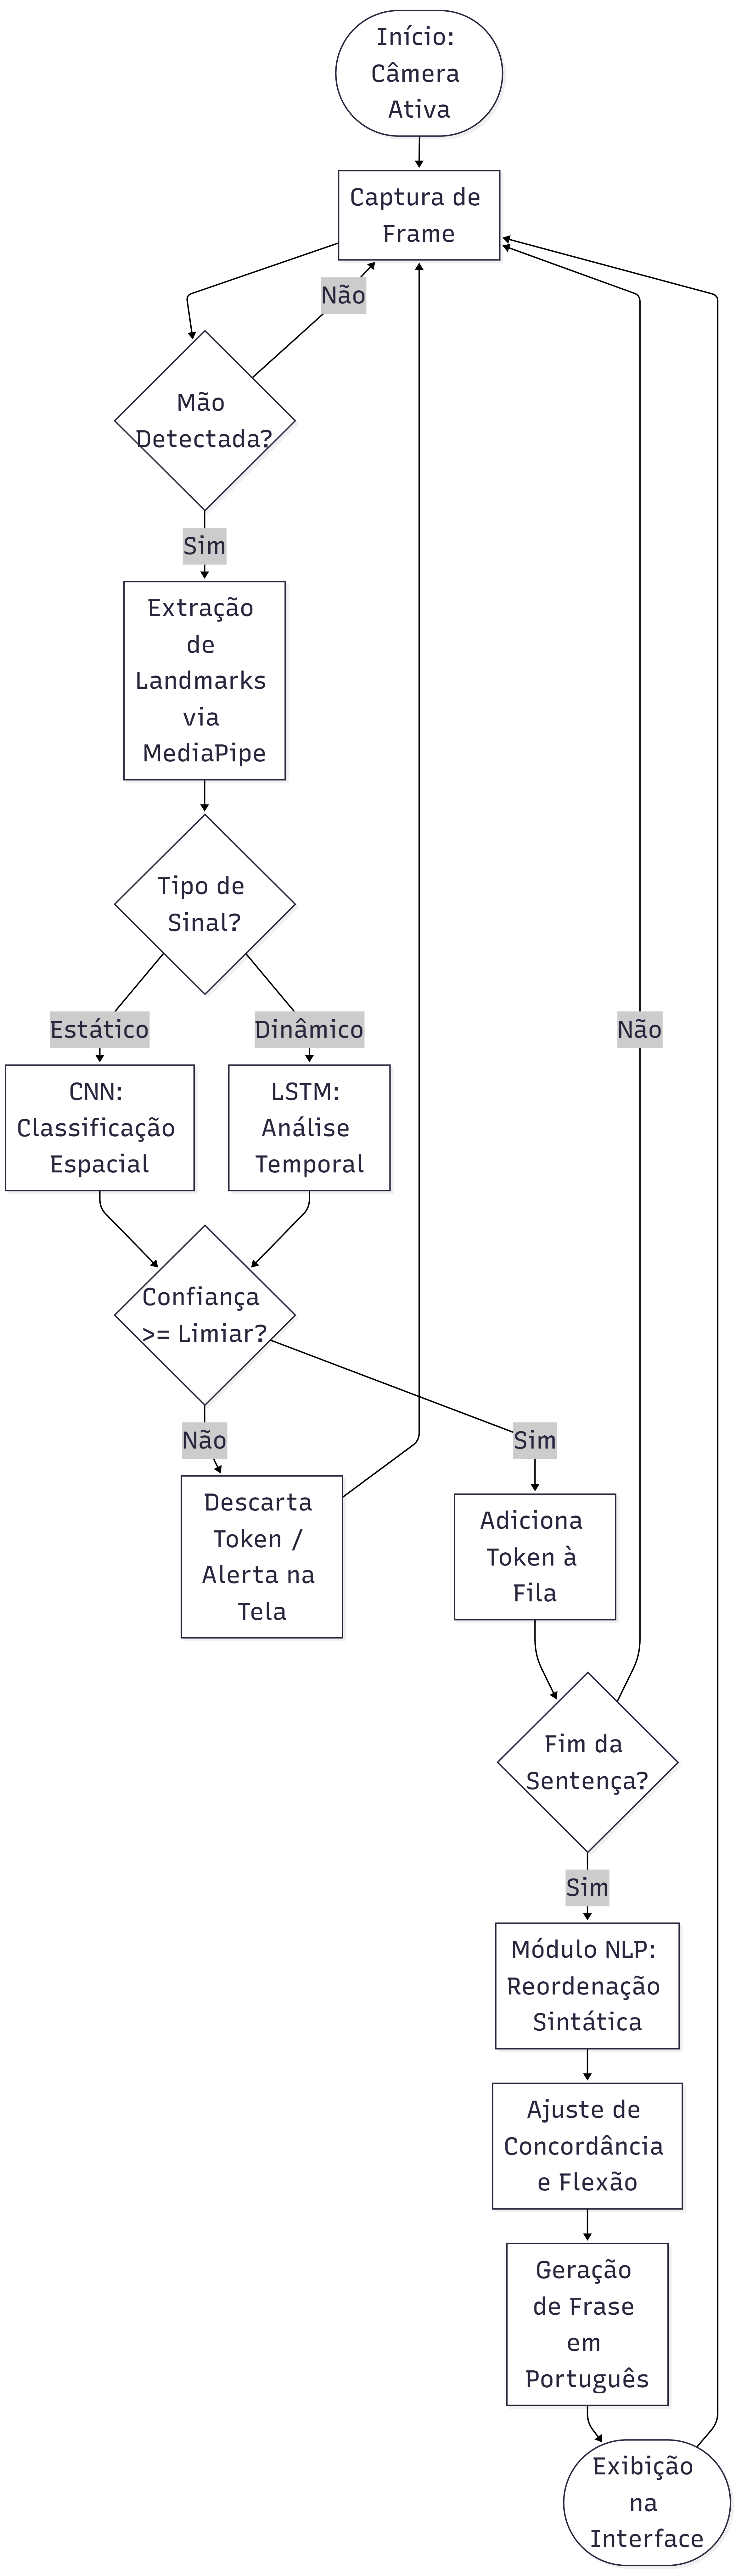
\includegraphics[width=0.4\textwidth]{./figuras/execução-pipeline}
    \caption{Fluxograma de Execução do Pipeline.}
    \source{Autoria própria (2026).}
\end{figure}
\subsection{Arquitetura}
A arquitetura do sistema é organizada de forma modular, dividida em três camadas principais de processamento que interagem sequencialmente para garantir a precisão da tradução:
\begin{enumerate}
    \item Camada de Aquisição e Visão (Front-end/Captura): Responsável por receber o fluxo de vídeo e utilizar algoritmos de extração de \textit{landmarks} para isolar os movimentos das mãos e do corpo.
    \item Camada de Inteligência (Processamento Híbrido): O núcleo da solução, onde Redes Neurais Convolucionais (CNN) processam a geometria espacial de cada frame e Redes de Memória de Longo Prazo (LSTM) interpretam a continuidade temporal dos movimentos.
    \item Camada de Interpretação Linguística (NLP): Módulo que recebe os sinais identificados (tokens) e aplica regras de Processamento de Linguagem Natural para gerar frases gramaticalmente corretas em língua portuguesa.
\end{enumerate}
\begin{figure}[H]
    \centering
    
\includegraphics[width=1.0\textwidth]{./figuras/visao-computacional.png}
    \caption{Fluxo de Processamento da Arquitetura Híbrida.}
    \source{Autoria própria (2026).}
\end{figure}
\subsection{Tecnologias e ferramentas}
As escolhas tecnológicas foram feitas visando o alto desempenho em processamento de tensores e visão computacional:
\begin{itemize}
    \item Linguagem de Programação: Python, devido à sua maturidade e vasta biblioteca para IA.
    \item Frameworks de Inteligência Artificial: TensorFlow ou Keras para o desenvolvimento das arquiteturas CNN e LSTM.
    \item Visão Computacional: MediaPipe ou OpenCV para a extração ágil de pontos de referência (\textit{landmarks}) das mãos.
    \item Dataset: Minds-Libras, Libras Brazilian Sign Language e V-BrasilIL escolhidos pela diversidade de sinais e qualidade das anotações.
    \item Processamento de Texto: Biblioteca NLTK ou spaCy para as tarefas de NLP e adequação gramatical.
\end{itemize}
\subsection{Funcionalidades principais}
Para atingir os objetivos propostos, o sistema disponibilizará as seguintes funcionalidades:
\begin{itemize}
    \item Captura de Sinais em Tempo Real: Processamento de vídeo via webcam com baixa latência.
    \item Reconhecimento de Sinais Estáticos e Dinâmicos: Capacidade de traduzir desde o alfabeto manual, como o da Figura~\ref{fig:alfabetoLibras}, até gestos complexos em movimento.
    \begin{figure}[H]
        \centering
        \caption{Alfabeto de Libras.} 
        \label{fig:alfabetoLibras}
        
\includegraphics[width=0.8\textwidth]{./figuras/alfabetoLibras.jpg}
        \fonte{\citeonline{Nascimento2018}.}
    \end{figure}
    \item Tradução Sintática Automática: Reorganização de sentenças da estrutura Libras para a estrutura SVO do português.
    \item Saída Multimodal: Exibição da tradução em texto na tela.
\end{itemize}
\subsection{Metodologia de desenvolvimento}
O projeto adotará a metodologia ágil Scrum, organizada em ciclos de desenvolvimento (Sprints). A escolha justifica-se pela natureza experimental de modelos de IA, permitindo testes contínuos e ajustes refinados nos hiperparâmetros das redes neurais a cada entrega parcial (prototipação).
\subsection{Critérios de validação}
O sucesso da solução será medido através de métricas quantitativas e qualitativas:
\begin{itemize}
    \item Acurácia e Precisão: Medição da taxa de acerto do modelo na classificação dos sinais utilizando uma matriz de confusão.
    \item Métrica BLEU (Bilingual Evaluation Understudy): Utilizada para avaliar a qualidade da tradução gerada pelo módulo de NLP em comparação com traduções humanas.
    \item Tempo de Resposta: Testes de latência para garantir que a tradução ocorra em tempo de execução.
\end{itemize}

% ---------------------------------------------------------------
\section{Cronograma de trabalho}
\label{sec:cronograma}

O cronograma a seguir apresenta, no formato de diagrama de Gantt, as atividades previstas para o desenvolvimento do TCC2, distribuídas ao longo das semanas do semestre.

\begin{figure}[htb]
    \centering
    \label{fig:gantt}
    % Resizebox ajusta o gráfico automaticamente à largura da página
    \resizebox{\textwidth}{!}{
        \begin{ganttchart}[
            hgrid,
            vgrid,
            x unit=0.6cm, % Reduzido para comprimir as semanas
            y unit title=0.6cm,
            y unit chart=0.6cm,
            title height=1,
            bar height=0.5,
            bar label font=\tiny, % Fonte menor para os nomes das tarefas
            title label font=\scriptsize,
            milestone label font=\tiny\itshape,
            group label font=\tiny\bfseries,
            bar/.append style={fill=blue!40},
            group/.append style={draw=black, fill=blue!70},
            milestone/.append style={fill=red!70},
        ]{1}{16}
            \gantttitle{Semanas}{16} \\
            \gantttitlelist{1,...,16}{1} \\

            \ganttgroup{Fase 1: Planejamento}{1}{4} \\
            \ganttbar{Revisão bibliográfica}{1}{2} \\
            \ganttbar{Requisitos do sistema}{2}{3} \\
            \ganttbar{Análise do dataset}{2}{4} \\
            \ganttbar{Projeto da arquitetura}{3}{4} \\
            \ganttmilestone{Entrega projeto}{4} \\

            \ganttgroup{Fase 2: Desenvolvimento}{5}{12} \\
            \ganttbar{Módulo Visão Computacional}{5}{7} \\
            \ganttbar{Treinamento CNN}{6}{8} \\
            \ganttbar{Implementação LSTM}{7}{9} \\
            \ganttbar{Desenvolvimento PLN}{8}{10} \\
            \ganttbar{Integração módulos}{10}{11} \\
            \ganttbar{Interface}{10}{12} \\
            \ganttmilestone{Protótipo}{12} \\

            \ganttgroup{Fase 3: Validação}{13}{16} \\
            \ganttbar{Testes e avaliação}{13}{14} \\
            \ganttbar{Ajustes e otimizações}{14}{15} \\
            \ganttbar{Redação final}{13}{16} \\
            \ganttmilestone{Entrega final}{16}

            \ganttlink{elem2}{elem3}
            \ganttlink{elem3}{elem4}
            \ganttlink{elem4}{elem5}
            \ganttlink{elem7}{elem8}
            \ganttlink{elem8}{elem9}
            \ganttlink{elem9}{elem10}
            \ganttlink{elem12}{elem13}
        \end{ganttchart}
    }
    \caption{Cronograma de atividades -- Diagrama de Gantt}
    \source{Autoria própria (2026).}
\end{figure}

% ---------------------------------------------------------------
% ELEMENTOS PÓS-TEXTUAIS
% ---------------------------------------------------------------
\postextual

% ===============================================================
% CAPÍTULO 4 - REFERÊNCIAS BIBLIOGRÁFICAS
% ===============================================================
% As referências bibliográficas são geradas automaticamente a partir
% do arquivo bibliografia.bib, seguindo o padrão ABNT (NBR 6023).
%
% COMO CITAR no texto:
%   \cite{chave}         -> (SOBRENOME, ano) — citação indireta
%   \citeonline{chave}   -> Sobrenome (ano) — citação direta no texto
%
% TIPOS DE REFERÊNCIA no arquivo .bib:
%   @book        -> Livros
%   @article     -> Artigos de periódicos
%   @inproceedings -> Artigos em anais de eventos
%   @mastersthesis -> Dissertações de mestrado
%   @phdthesis   -> Teses de doutorado
%   @misc        -> Sites, vídeos e outros materiais
%   @manual      -> Documentação técnica
%
% Veja o arquivo bibliografia.bib para exemplos de cada tipo.
% ---------------------------------------------------------------

\bibliography{bibliografia}

% ---------------------------------------------------------------
% APÊNDICES (se necessário)
% ---------------------------------------------------------------
% \begin{apendicesenv}
% \partapendices
%
% \chapter{Nome do Apêndice}
% \label{ap:apendice1}
%
% Conteúdo do apêndice (material elaborado pelo próprio autor).
%
% \end{apendicesenv}

% ---------------------------------------------------------------
% ANEXOS (se necessário)
% ---------------------------------------------------------------
% \begin{anexosenv}
% \partanexos
%
% \chapter{Nome do Anexo}
% \label{an:anexo1}
%
% Conteúdo do anexo (material de terceiros).
%
% \end{anexosenv}

\end{document}
